\documentclass[12pt]{article}
\usepackage[brazil]{babel}
\usepackage[a4paper, total={6.5in, 9.5in}]{geometry}
\usepackage[utf8]{inputenc}
\usepackage[T1]{fontenc}
\usepackage{listings}
\usepackage{xcolor}
\usepackage{float}
\usepackage{graphicx}

\definecolor{codegreen}{rgb}{0,0.6,0}
\definecolor{codegray}{rgb}{0.5,0.5,0.5}
\definecolor{codered}{rgb}{0.8,0,0}
\definecolor{backcolour}{rgb}{0.95,0.95,0.92}

\usepackage{inconsolata}
\lstset{
    language=sql,
    backgroundcolor=\color{backcolour},   
    commentstyle=\color{codegreen},
    keywordstyle=\color{blue},
    numberstyle=\tiny\color{codegray},
    stringstyle=\color{codered},
    basicstyle=\ttfamily\small,
    numberstyle=\footnotesize,
    numbers=left,
    backgroundcolor=\color{gray!10},
    frame=single,
    tabsize=2,
    rulecolor=\color{black!30},
    title=\lstname,
    escapeinside={\%*}{*)},
    breaklines=true,
    breakatwhitespace=true,
    framextopmargin=2pt,
    framexbottommargin=2pt,
    inputencoding=utf8,
    extendedchars=true,
    showstringspaces=false,
    literate={á}{{\'a}}1 {ã}{{\~a}}1 {é}{{\'e}}1 {Ó}{{\'O}}1 {Ã}{{\~A}}1 {í}{{\'i}}1 {ó}{{\'o}}1,
}

\title{Projeto Final}
\author{Pedro Henrique de Brito Agnes, 18/0026305 \\
Pedro Pessoa Ramos, 180026488}
\date{}

\begin{document} 
\maketitle

\section*{Introdução}

Para o projeto final da disciplina de Banco de Dados, foi desenvolvido um software para auxiliar o professor no modelo de aulas remotas

\begin{lstlisting}
-- lista de todas as pessoas cadastradas (professores e alunos)
select	* from pessoas
\end{lstlisting}

\begin{figure}[H]
	\centering
    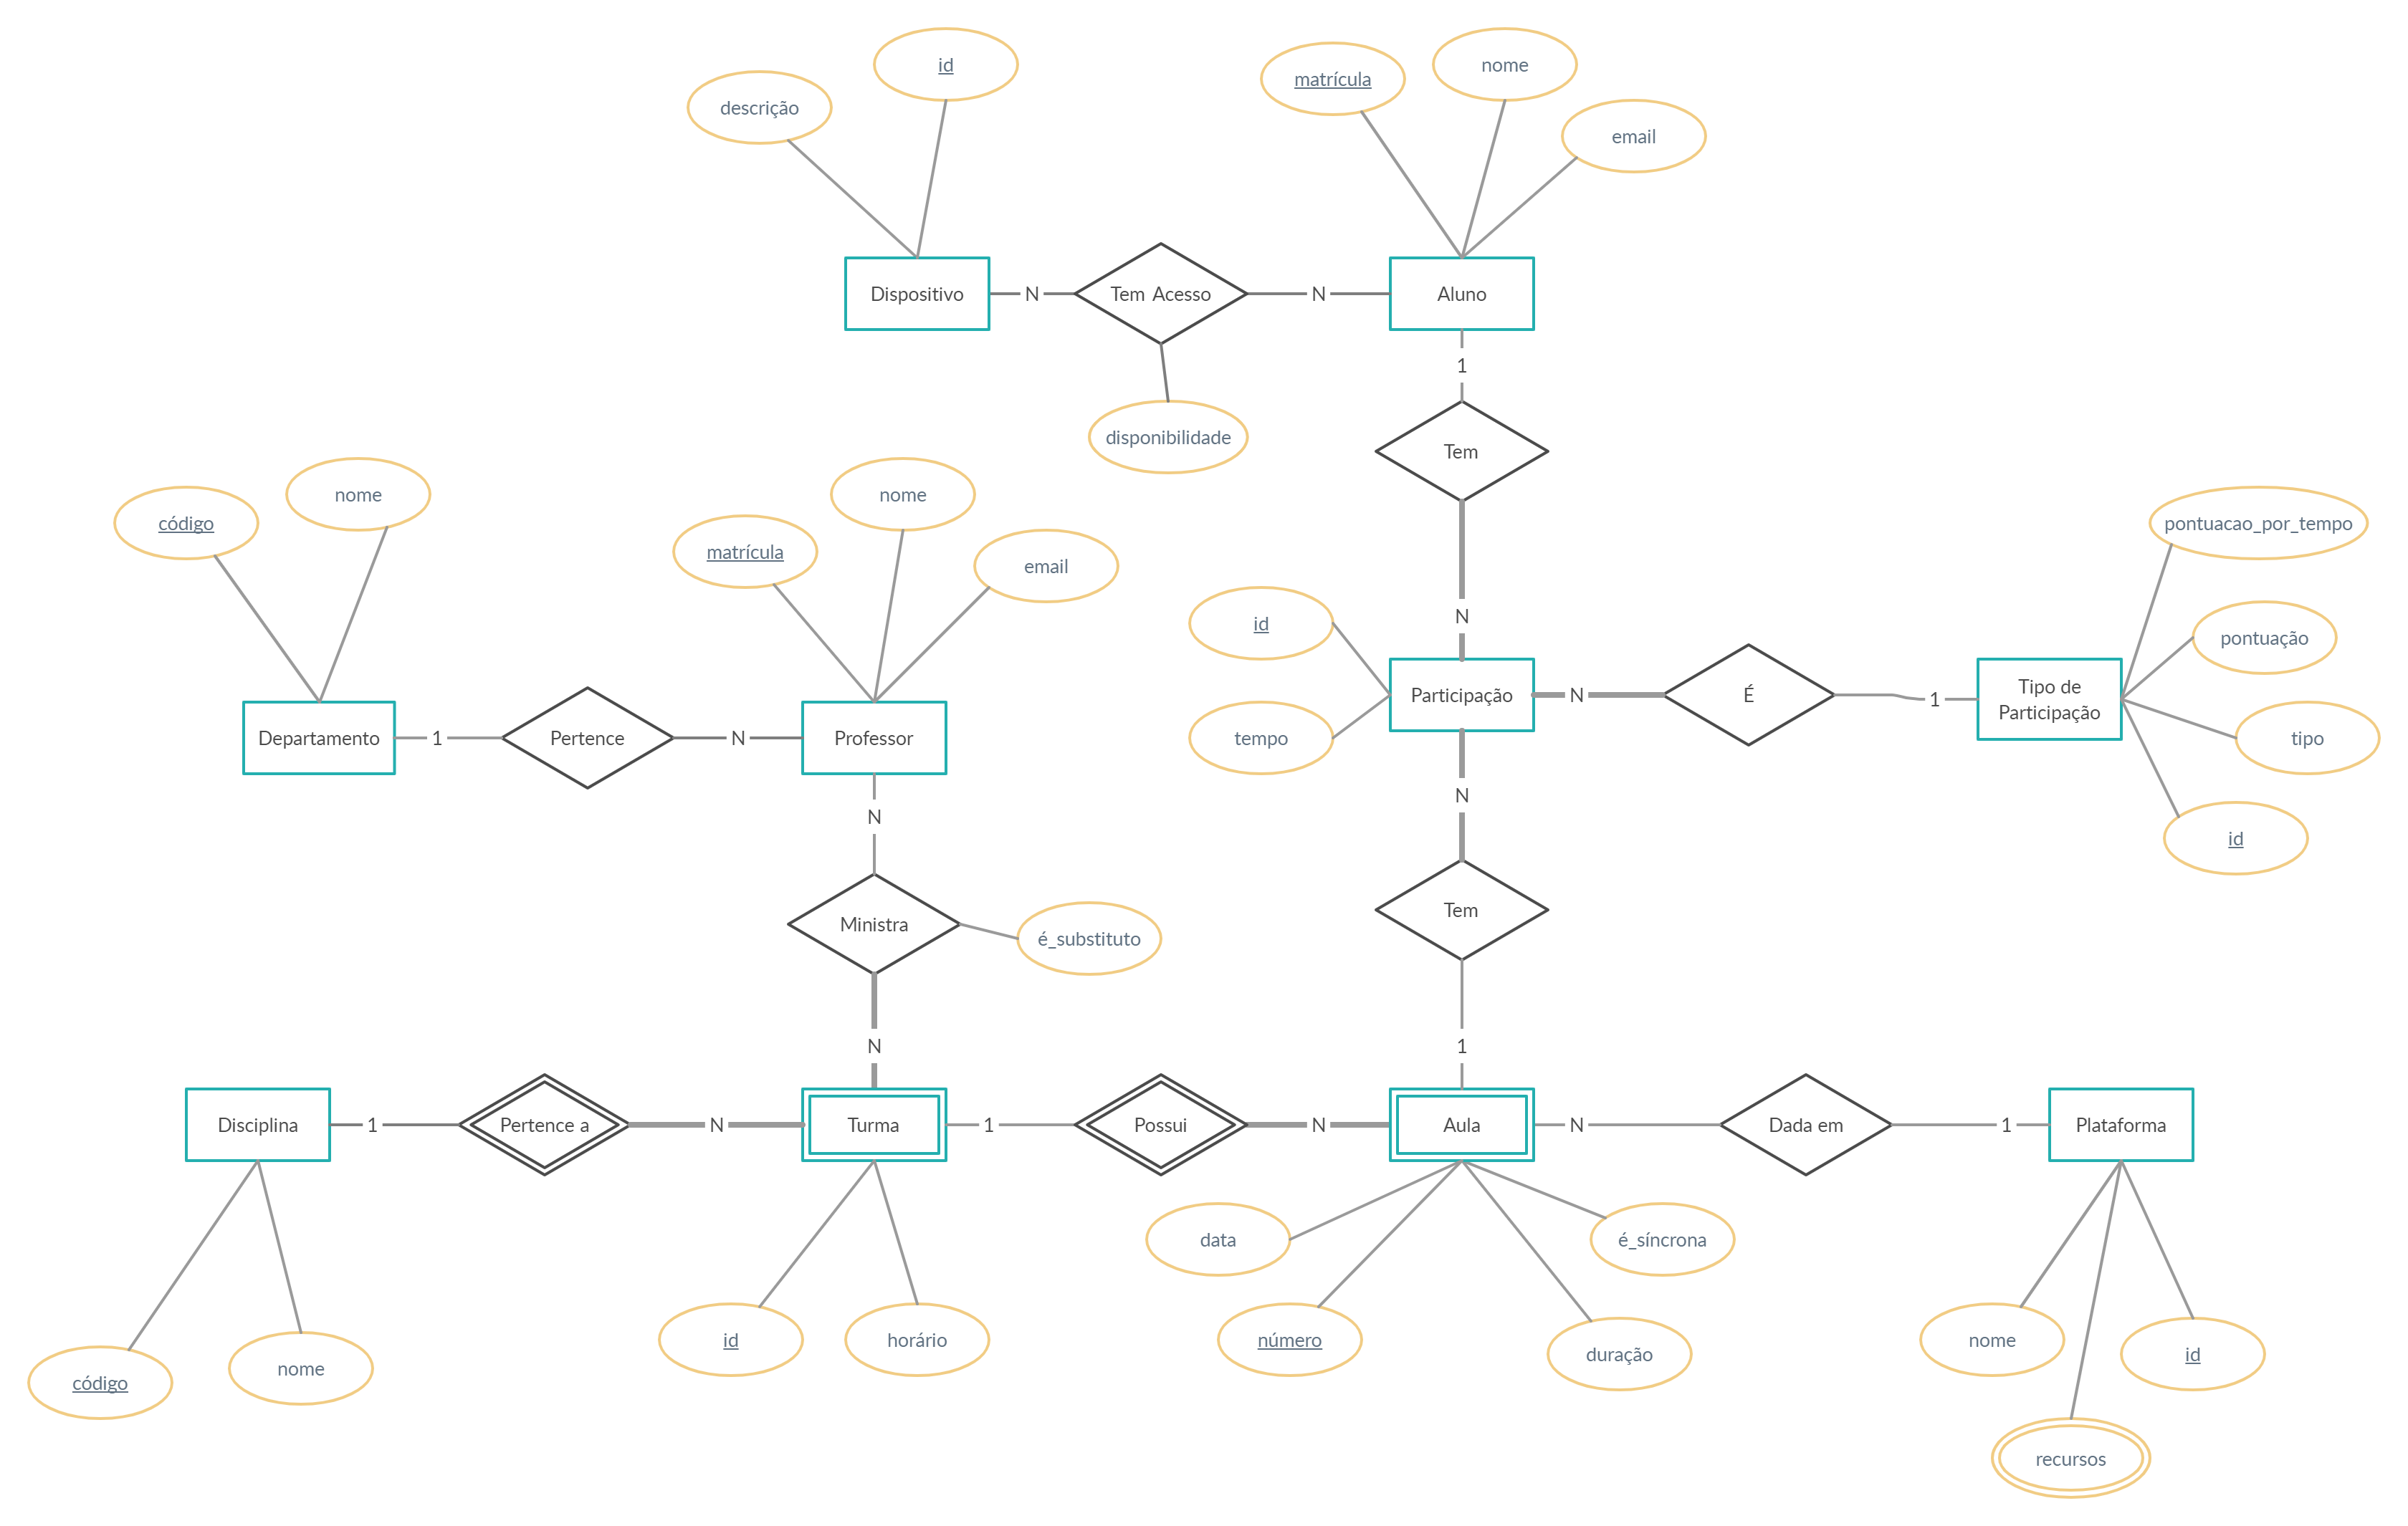
\includegraphics[width=1\textwidth]{MER.png}
    \caption{Modelo Entidade Relacionamento}
\end{figure}

\end{document}
